
\section{Use Cases and Evaluation}

As of today, we have mostly evaluated the iFLUX from a developer's point of view. We have looked at the following questions: how easy is it to grasp the programming model? How easy is it to create a new service or to expose a legacy service through iFLUX APIs? How easy is it to build an application by applying the programming model? To answer these questions, we have worked with various teams to develop both components and applications. These teams had no prior knowledge about iFLUX before starting the exercise. In all cases, we saw that it was easy and quick both to implement iFLUX APIs in existing components and to design end-to-end workflows.

\begin{figure*}
\centering
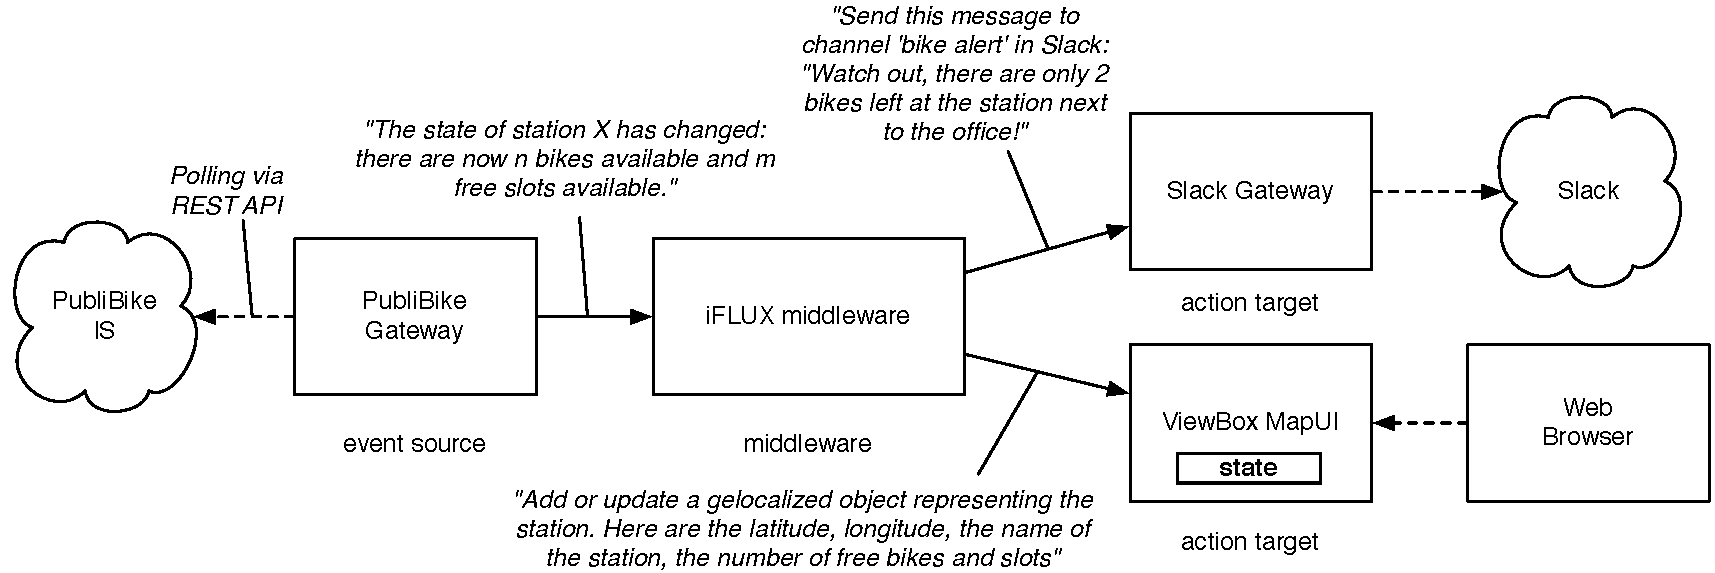
\includegraphics[width=0.7\textwidth]{figures/publibike.pdf}
\caption{The PubliBike application, with one event source and two action targets}
\label{fig:publibike}
\end{figure*}

\begin{figure*}
\centering
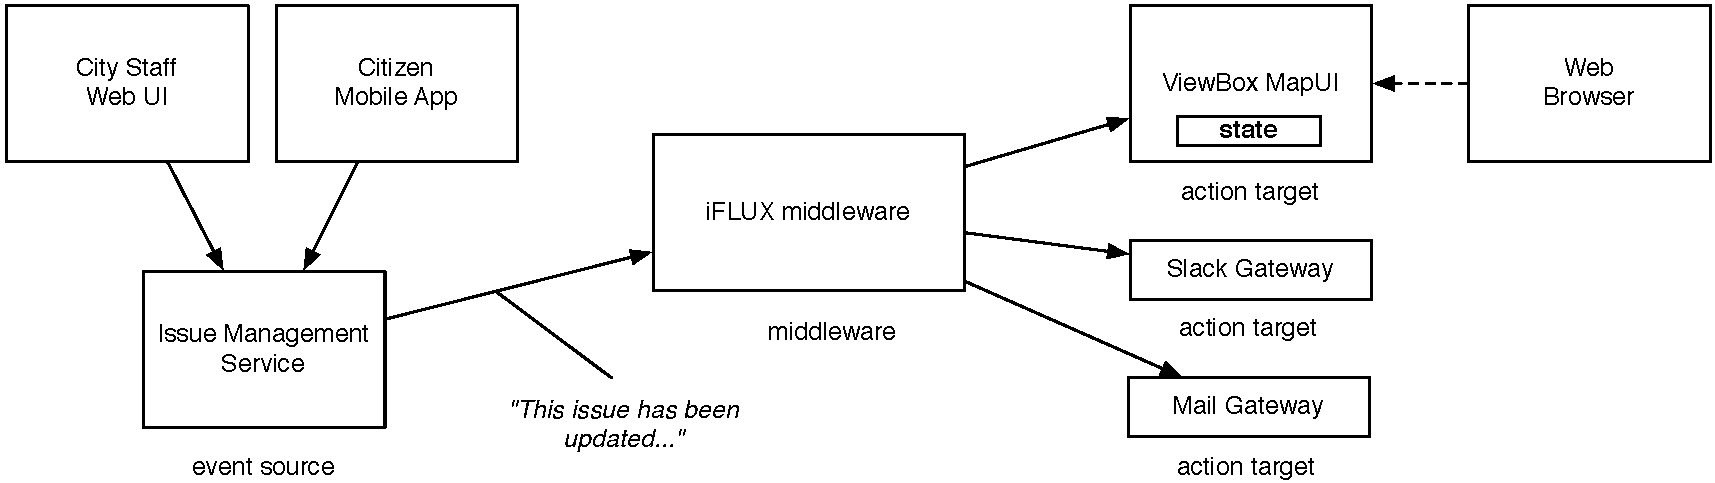
\includegraphics[width=0.7\textwidth]{figures/citizen}
\caption{The Citizen Engagement application, with one event source and three action targets}
\label{fig:citizen}
\end{figure*}

%\begin{figure*}
%\centering
%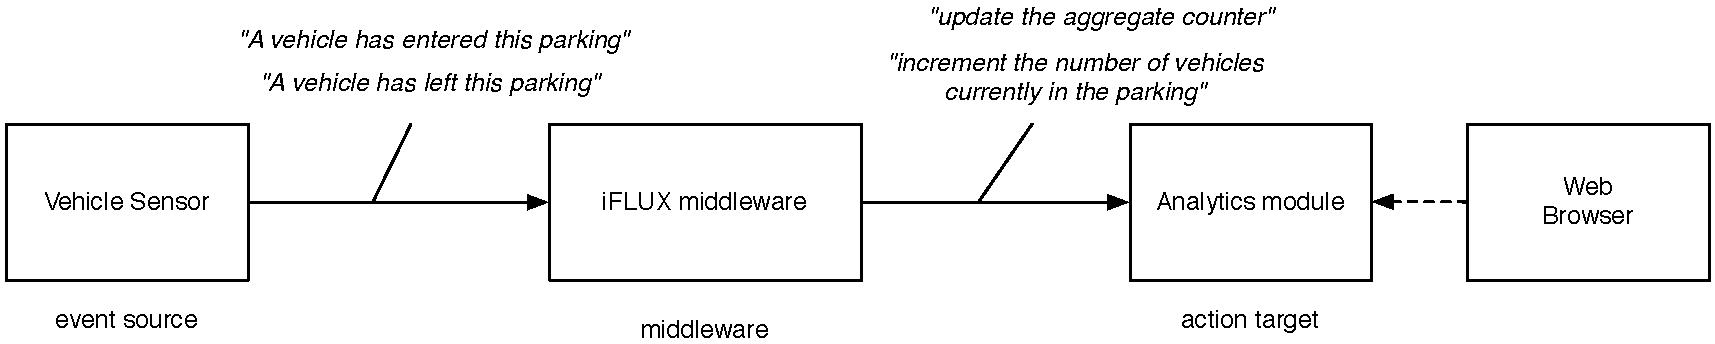
\includegraphics[width=0.9\textwidth]{figures/paleo}
%\caption{The Paléo Festival application, with one event source and one action target}
%\label{fig:paleo}
%\end{figure*}

%\begin{figure*}
%\centering
%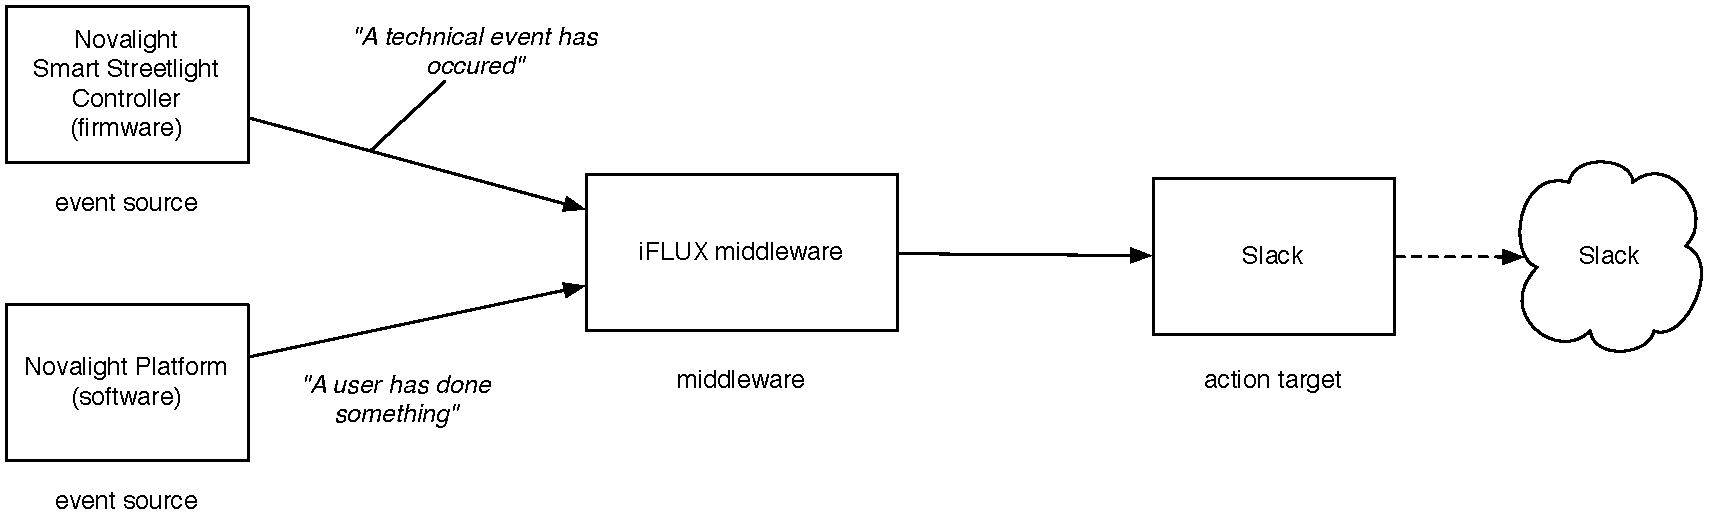
\includegraphics[width=0.9\textwidth]{figures/awareness}
%\caption{The Awareness @ Novaccess application, with two event sources and one action target}
%\label{fig:paleo}
%\end{figure*}


\subsection{PubliBike}

Like in many other countries, bike sharing stations are increasingly deployed in swiss cities (see Figure \ref{fig:publibikeStation}). Customers need to acquire a smart card, with which they can unlock a bike at a station. They also use the smart card when they later return the bike. The bike stations are connected to a nation-wide information system, named PubliBike. PubliBike makes it possible to know the number of available bikes and free slots at every station, in realtime. The data can be accessed via a REST API: the returned JSON payload contains the current state of all stations.

\begin{figure}[H]
\centering
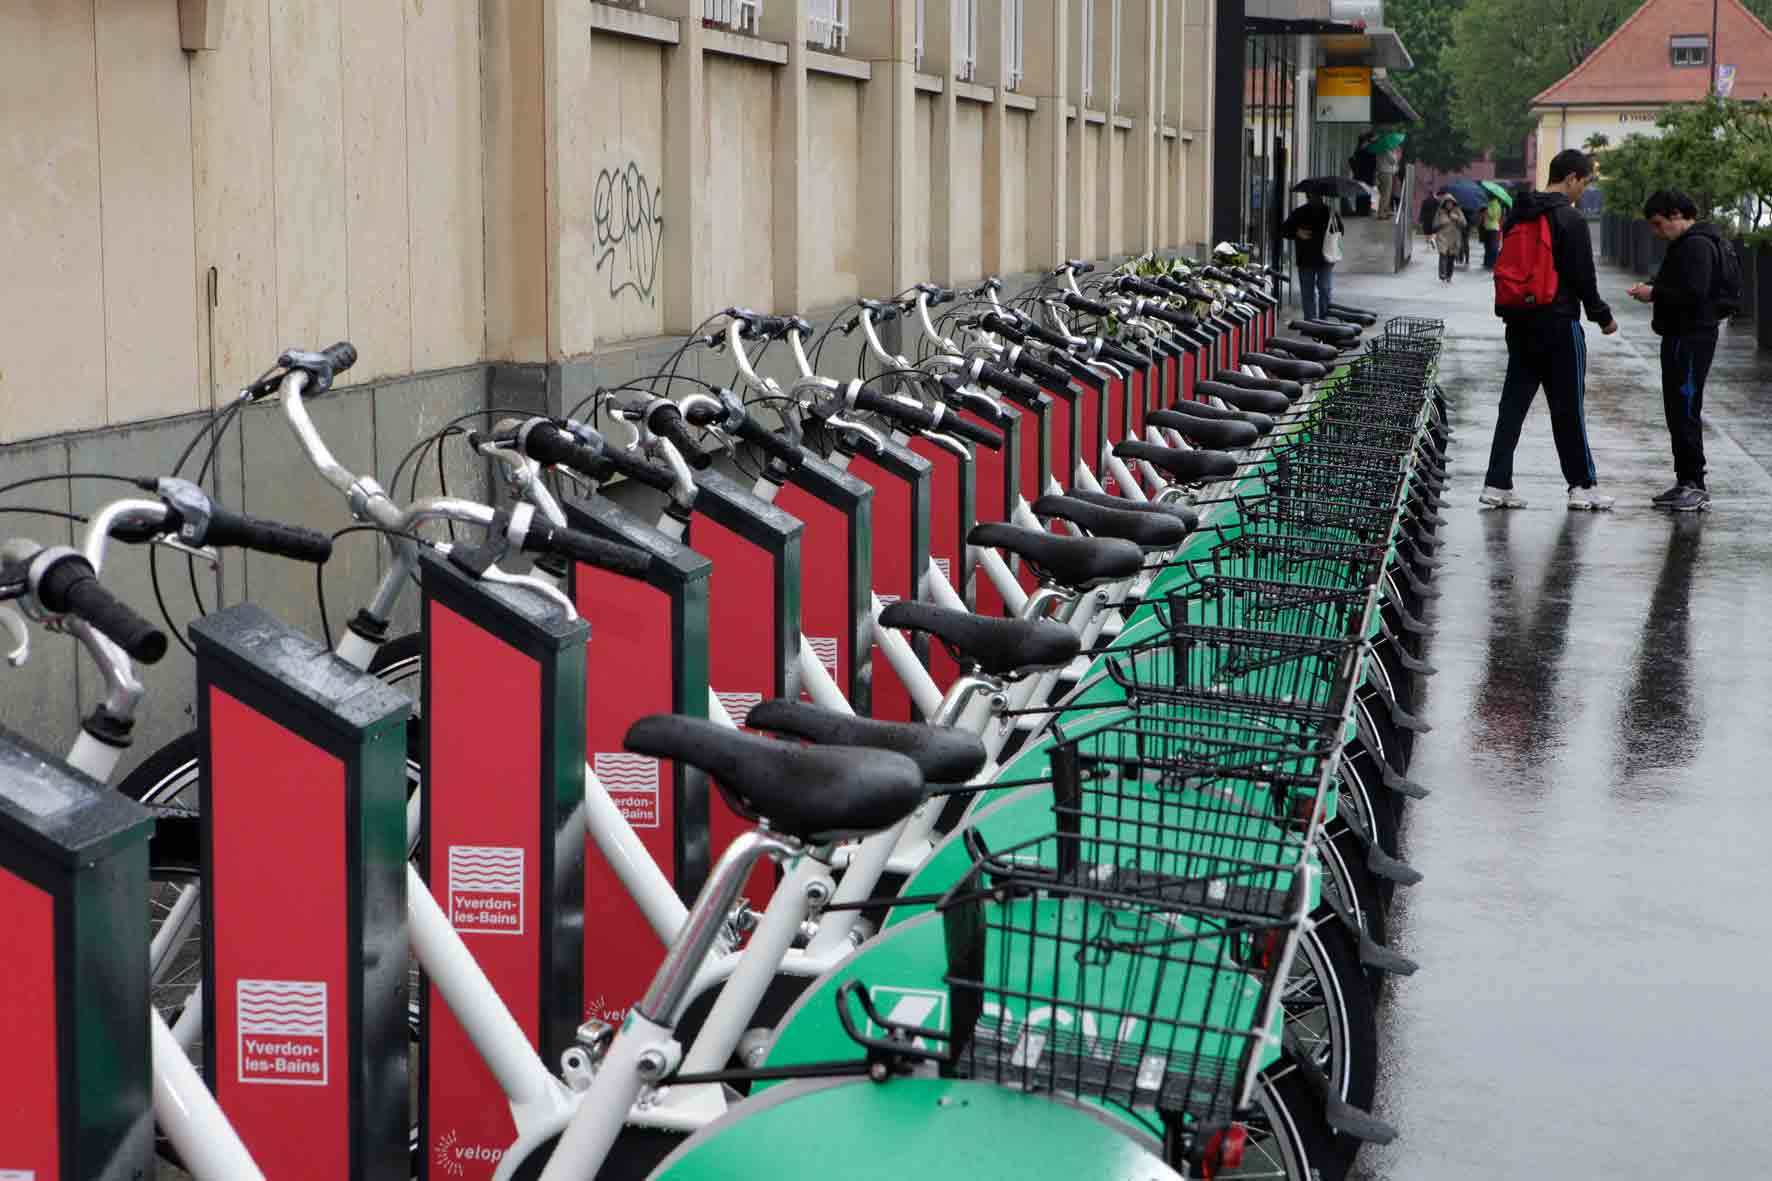
\includegraphics[width=0.85\columnwidth]{figures/publibikephoto2.jpg}
\caption{A bike station in Yverdon-les-Bains}
\label{fig:publibikeStation}
\end{figure}

\begin{figure}[H]
\centering
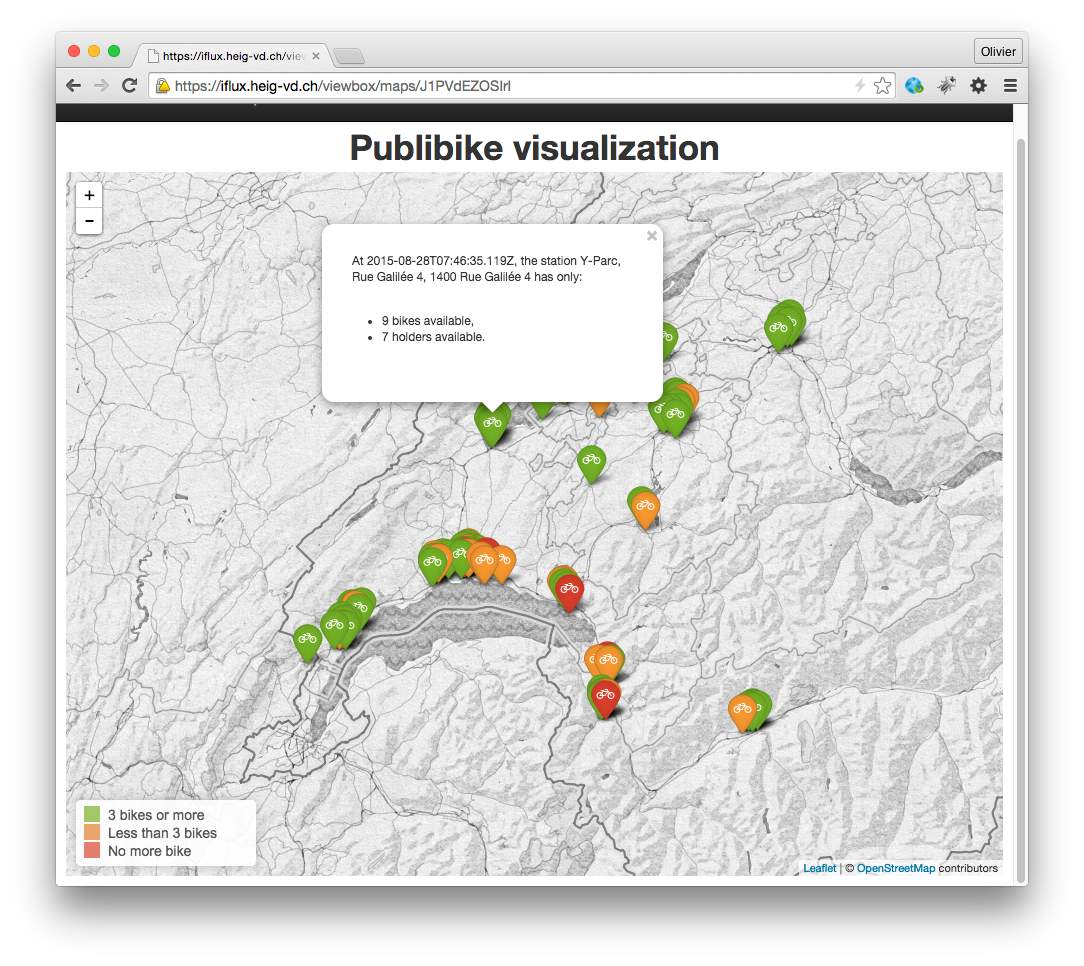
\includegraphics[width=0.75\columnwidth]{figures/publibike-viewbox.png}
\caption{Bike stations displayed by an action target}
\label{fig:publibikeMap}
\end{figure}


As illustrated in Figure \ref{fig:publibike}, we have implemented one \emph{event source} and two \emph{action targets} and we have defined rules in order to react to the activity monitored within the PubliBike system. These components are described in the following paragraphs.

\subsubsection{Tracking bike arrival and departure: the PubliBike Event Source}
Integrating PubliBike into the iFLUX ecosystem has first been achieved by defining a new \emph{event source} and by specifying the type of events produced by this source. Note that when doing this, we did not need to think about how the information would be used. It could be used to trigger alerts, to create visual representations, to compute statistics. As developers of the \emph{event source}, this is not something that we had to worry about (decoupling). We could have decided to define one \emph{event source} for every bike station, but instead we have preferred to define a single \emph{event source}: the PubliBike gateway, which is responsible for polling data via the PubliBike API and to detect state changes. In this scenario, while there are sensors and communication modules embedded in the physical stations, the iFLUX \emph{event source} is purely implemented in a software daemon running in the cloud. With the PubliBike \emph{event source} deployed, iFLUX receives an incoming stream of events, where every event represents a state change at a given station (i.e. either a bike has arrived or left). In addition to a timestamp, the events contain the following properties: the identifier, name and geographic coordinates of the station, the number of available bikes and the number of free slots. 

To setup the \emph{event source} we have started by configuring the \emph{event source template}. As we discussed earlier, the event source template allows us to create multiple event source of the same kind. In this case, we want to have only one \emph{event source}. We want to configure the system to have our Publibike \emph{event source} as a sort of singleton. For that, we create the \emph{event source template} to be private in our organization and then we create the \emph{event source} to be public. Therefore, we offer to users of different organizations the possibility to create rules with our Publibike \emph{event source} but we forbid to create new \emph{event sources}. The limitation is if a member of our organization create a second \emph{event source} from the template. We cannot avoid that at the moment. A future evolution of the system can be to set a flag or a counter to limit the number of \emph{event sources} from a template.

Now, let's take a look of what we send on our API to create the \emph{event source template}. We can see that we just set a name, the public flag to false and we attach it to our organization.

\begin{lstlisting}
POST /eventsourcetemplates HTTP/1.0
Content-Type: application/json

{
  "name": "Publibike",
  "public": false,
  "organizationId": 1
}
\end{lstlisting}

For the \emph{event source}, we have to send the following

\begin{lstlisting}
POST /eventsources HTTP/1.0
Content-Type: application/json

{
  "name": "Publibike singleton data poller"
  "eventSourceTemplateId": 1,
  "organizationId": 1,
  "public": true
}
\end{lstlisting}

We also need to define which kind of events the source will send. We create an event type to notify the state of a bike station with the remaining bikes and free slots before and after the event is occurring. This is how we create the \emph{event type} through our API. With the \emph{event type} public, we let other users in iFLUX to use the definition of the event type for different usage. Defining the \emph{event type} will let the rule creators to know which data he will receive in an event of that type.

\begin{lstlisting}
POST /eventtypes HTTP/1.0
Content-Type: application/json

{
  "name": "Publibike status event",
  "description": "State of a Publibike station when one or more bikes left/arrived.",
  "public": "true",
  "type": "http://localhost.localdomain/eventTypes/publibikeMovement",
  "schema": {
    "$schema": "http://json-schema.org/draft-04/schema#",
    "type": "object",
    "properties": {
      "terminalid": { "type": "string" },
      "terminal": {
        "type": "object",
        "properties": {
          "name": { "type": "string" },
          "infotext": { "type": "string" },
          "zip": { "type": "string" },
          "city": { "type": "string" },
          "country": { "type": "string" },
          "lat": { "type": "string" },
          "lng": { "type": "string" },
          "image": { "type": "string" },
        }
      },
      "old": {
        "type": "object",
        "properties": {
          "freeholders": { "type": "integer" },
          "bikes": { "type": "integer" }
        }
      },
      "new": {
        "type": "object",
        "properties": {
          "freeholders": { "type": "integer" },
          "bikes": { "type": "integer" }
        }
      }
    }
  }
}
\end{lstlisting}

\subsubsection{Notifying users: the Slack action target}
Someone who uses the bike sharing service to commute from the office to the train station might be interested to be notified if the number of available bikes close to the office falls below a certain threshold. This person might also be interested to receive an alert if the number of free slots at the station falls below a threshold. To implement this use case, the user needs an iFLUX \emph{action target} that provides a bridge to a notification system (SMS, e-mail, etc.). To illustrate the idea, we have implemented an action target that makes it possible to send a notification in the Slack instant messaging platform \cite{slack}. The payloads sent to the action target via the REST API contain the message and the name of the channel where to post it. 

We start to define the \emph{action target template} which represent the Slack Gateway. The bot who will send the messages is configurable and then the \emph{action target} represent this bot configuration. So we make our \emph{action target template} public to let other users to use the gateway in a different context with the correct configuration. We can observe that we define the configuration part. This will let the user to provide the correct configuration that will be applied by posting the configuration on the callback URL of the remote action target.

\begin{lstlisting}
POST /actiontargettemplates HTTP/1.0
Content-Type: application/json

{
  "name": "iFLUX Slack Gateway",
  "public": true,
  "organizationId": 1,
  "configuration": {
    "schema": {
      "$schema": "http://json-schema.org/draft-04/schema#",
      "type": "object",
      "properties": {
        "token": {
          "type": "string"
        }
      },
      "additionalProperties": false,
      "required": [ "token" ]
    },
    "url": "http://localhost.localdomain/configure"
  },
  "target": {
    "url": "http://localhost.localdomain/actions"
  }
}
\end{lstlisting}

And we define the \emph{action target} for the context of Publibike. We set the configuration that will be applied on the remote action target. In our case, the token is given by Slack to do the authentication when we send a message from our action target to Slack.

\begin{lstlisting}
POST /actiontargets HTTP/1.0
Content-Type: application/json

{
  "name": "Publibike slack messages",
  "organizationId": 1,
  "actionTargetTemplateId": 1,
  "public": true,
  "configuration": {
    "token": "<theSlackTokenToAuthentifyTheBot>"
  }
}
\end{lstlisting}

Finally, we need to define the \emph{action type} to know what is the JSON payload that the \emph{action target} will accept. There is the \emph{action type} used in this case.

\begin{lstlisting}
POST /actiontypes HTTP/1.0
Content-Type: application/json

{
  "name": "Slack message",
  "public": true,
  "type": "http://localhost.localdomain/actionTypes/slackMessageSending",
  "schema": {
    "$schema": "http://json-schema.org/draft-04/schema#",
    "type": "object",
    "properties": {
      "message": {
        "type": "string"
      },
      "channel"; {
        "type": "string"
      }
    }
  }
}
\end{lstlisting}

We have all the pieces in place to define a simple rule. There is an example below where we simply send Slack messages with the state of the bike stations every time an event occurs. There is the rule we define for that.

\begin{lstlisting}
POST /rules HTTP/1.0
Content-Type: application/json

{
  "name": "Publibike movements",
  "description": "Broadcast Publibike changes at a bike station to Slack.",
  "active": true,
  "organizationId": 1,
  "conditions": [{
    "description": "Detect the arrival or the departure of one or more bikes at a station",
    "eventTypeId": 1
  }],
  "transformations": [{
    "description": "Send a message to Slack",
    "actionTargetId": 1,
    "actionTypeId": 1,
    "fn": {
      "expression": "return { channel: 'iflux', message: 'Only ' + event.properties.new.bikes + ' bike(s) available at the station ' + event.properties.terminal.name + ', ' + event.properties.terminal.street + ', ' + event.properties.terminal.zip + ' ' + event.properties.terminal.city + '.' };",
      "sample": {
	"eventSourceTemplateId": 1,
        "event": {
          "terminalid": "asdfghjkl",
          "terminal": {
            "name": "Y-Parc",
            "infotext": "Parc Scientifique - Yverdon",
            "zip": "1400",
            "city": "Yverdon-les-Bains",
            "country": "Switzerland",
            "lat": 46.764968,
            "lng": 6.646069,
            "image": ""
          },
          old: {
            "freeholders": 10,
            "bikes": 3
          },
          "new": {
            "freeholders": 11,
            "bikes": 2
          }
        }
      }
    }
  }]
}
\end{lstlisting}

With this setup, a user can define other iFLUX rules. For example, he can define a rule which states that \emph{\textbf{IF} an event is received from the PubliBike event source AND the event property `terminalId' of the event is the one of the station close to my office AND if the event property `new.bikes' is less than 3 \textbf{THEN} send an action to the Slack action target, with the property `channel' set to `bike alerts' and the property `message' set to `WARNING: there are not many bikes left at the station!'}. 

\subsubsection{Map visualization: the ViewBox action target}
Another idea for using the data produced by the PubliBike event source was to create a visual representation, where the current state of every bike station is shown on a geographical map (see Figure \ref{fig:publibikeMap}). This use case is interesting, because it raises the question about how to deal with application state given that iFLUX rules are stateless.

We have implemented an \emph{action target} that we have named the \emph{ViewBox action target}. Note that while it can be used in conjunction with the \emph{PubliBike event source}, it is generic and can be used with other types of \emph{event sources} (for instance, it has been used in the citizen engagement application described later). Essentially, the \emph{ViewBox action target} is responsible for managing application state, which is defined by a collection of geolocalized objects, which can have arbitrary properties attached to them. It accepts action payloads with the following properties: the unique identifier of a geolocalized object, the current latitude and longitude and a list of application specific values (in the case of PubliBike, the name of the station and the number of available bikes and slots). When it receives an action via the REST endpoint, it creates or updates a geolocalized object with the property values in the payload. The \emph{action target} provides its own API (outside the scope of iFLUX), so that web browsers can fetch annotated maps. 

After deploying the \emph{Viewbox action target}, we were able to configure a rule so that whenever an event was received from the \emph{PubliBike event source}, an action would be sent to the \emph{ViewBox action target} to update the corresponding geolocalized object.

To achieve the setup for the \emph{Viewbox} visualization, we created the \emph{action target template} which define configuration to contextualize the usage of the action target.

\begin{lstlisting}
POST /actiontargettemplates HTTP/1.0
Content-Type: application/json

{
  "name": "iFLUX ViewBox",
  "organizationId": 1,
  "public": true,
  "configuration": {
    "schema": {
      "$schema": "http://json-schema.org/draft-04/schema#",
      "type": "object",
      "properties": {
        "mapName": { "type": "string" },
        "expiration": { "type": "integer" },
        "mapConfig": {
          "type": "object",
          "properties": {
            "centerLat": { "type": "number" },
            "centerLng": { "type": "number" },
            "initialZoom": { "type": "integer" },
            "legendType": { "type": "string" }
          },
          "required": [ "centerLat", "centerLng", "initialZoom", "legendType" ]
        }
      },
      "additionalProperties": false,
      "required": [ "mapName", "mapConfig" ]
    },
    "url": "http://localhost.localdomain/configure"
  },
  "target": {
    "url": "http:/localhost.localdomain/actions"
  }
}
\end{lstlisting}

And the \emph{action target} for the Publibike use case. We setup the map configuration to let the visual representation to be customized for this use case. On the \emph{ViewBox} instance, it will create a new map visualization dedicated for Publibike. The state of the markers on the map will managed and the data older than 24h will be discarded.

\begin{lstlisting}
POST /actiontypes HTTP/1.0
Content-Type: application/json

{
  "name": "iFLUX ViewBox Publibike Instance",
  "actionTargetTemplateId": 2,
  "organizationId": 1,
  "configuration": {
    "mapName": "Publibike visualization",
    "expiration": 86400000,
    "mapConfig": {
      "centerLat": 46.801111,
      "centerLng": 8.226667,
      "initialZoom": 9,
      "legendType": "bike"
    }
  }
}
\end{lstlisting}

Finally, there is the rule configured on iFLUX to match the Publibike events and trigger the Viewbox actions.

\begin{lstlisting}
POST /rules HTTP/1.0
Content-Type: application/json

{
  "name": "Publibike visualization",
  "description": "Update a map with the bike stations markers with their state.",
  "active": true,
  "organizationId": 1,
  "conditions": [{
    "description": "Detect bike movements",
    "eventTypeId": 1
  }],
  "transformations": [{
    "description": "Notify a change in station to update the visualization.",
    "actionTargetId": 2,
    "actionTypeId": 2,
    "fn": {
      "expression": "return { markerId: event.properties.terminal.terminalid, lat: event.properties.terminal.lat, lng: event.properties.terminal.lng, date: event.timestamp, data: { type: 'bike', name: event.properties.terminal.name, street: event.properties.terminal.street, city: event.properties.terminal.street, zip: event.properties.terminal.zip, freeholders: event.properties.new.freeholders, bikes: event.properties.new.bikes }};",
      "sample": {
	"eventSourceTemplateId": 1,
        "event": {
          "terminalid": "asdfghjkl",
          "terminal": {
            "name": "Y-Parc",
            "infotext": "Parc Scientifique - Yverdon",
            "zip": "1400",
            "city": "Yverdon-les-Bains",
            "country": "Switzerland",
            "lat": 46.764968,
            "lng": 6.646069,
            "image": ""
          },
          old: {
            "freeholders": 10,
            "bikes": 3
          },
          "new": {
            "freeholders": 11,
            "bikes": 2
          }
        }
      }
    }
  }]
}
\end{lstlisting}

With a different configuration in the rules, we can imagine to maintain different maps. For example, we can imagine to create a rule to visualize dedicated cities like Lausanne, Zurich where there are enough bike stations.

%\FloatBarrier



\subsection{Citizen Engagement}

After a few months of work on iFLUX, we used the platform in a two-weeks undergraduate course dedicated to end-to-end mobile services. The course is project-oriented and every year, we use an application domain to provide some context to the students. This year, we explained that software platforms are increasingly deployed, so that citizen can report issues to city authorities \cite{patel2015guide,offenhuber2014infrastructure}. Users can report broken street lights, graffitis, dangerous areas, etc. The students were asked to design a system with two components. Firstly, they had to implement a simple issue tracking system and to expose their domain model via a RESTful API. Secondly, they had to implement a mobile app that would be provided to citizen, so that they could easily report issues and follow their resolution process. You can see an illustration in Figure \ref{fig:citizenMobile}.

\begin{figure}
\centering
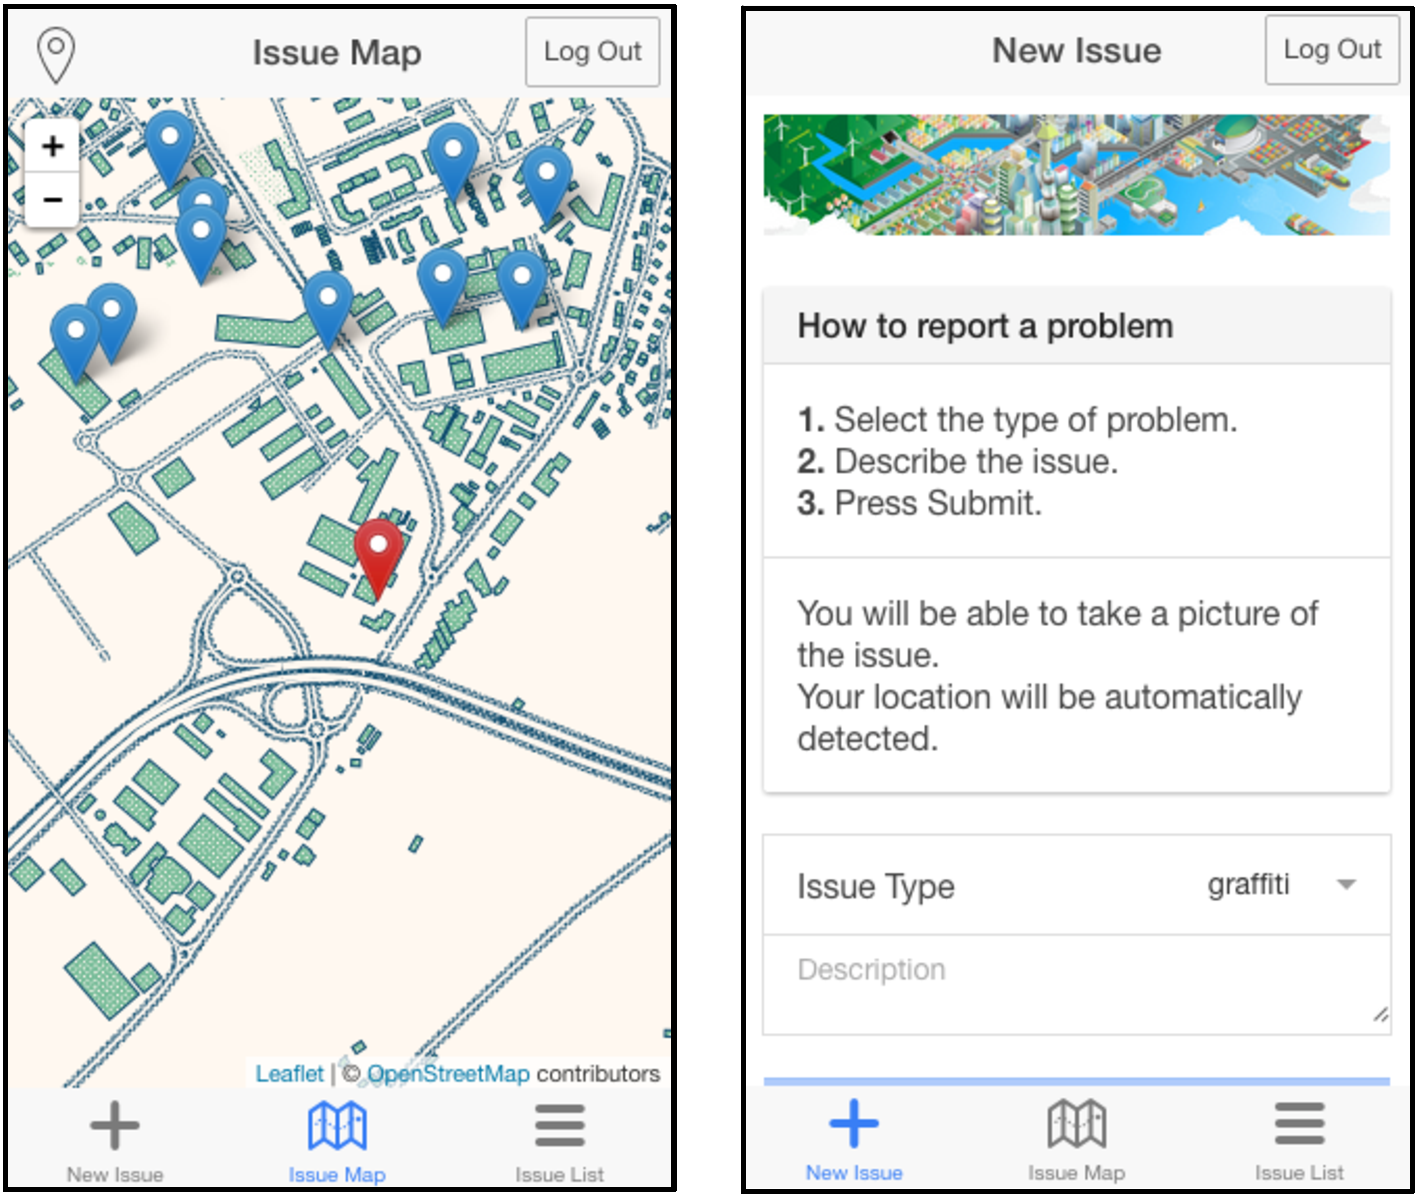
\includegraphics[width=0.8\columnwidth]{figures/citizen-mobile.pdf}
\caption{The mobile app used to report issues}
\label{fig:citizenMobile}
\end{figure}


The Citizen Engagement back-end was then transformed into an iFLUX \emph{event source}. This was done by emitting an event whenever the state of an issue would change (created, acknowledged, in progress, resolved, etc.). Special properties were added to the event (e.g. to attach comments to state transitions). Again, since emitting an iFLUX event is not more complicated than issuing a POST request, the integration was trivial. 

\begin{figure}
\centering
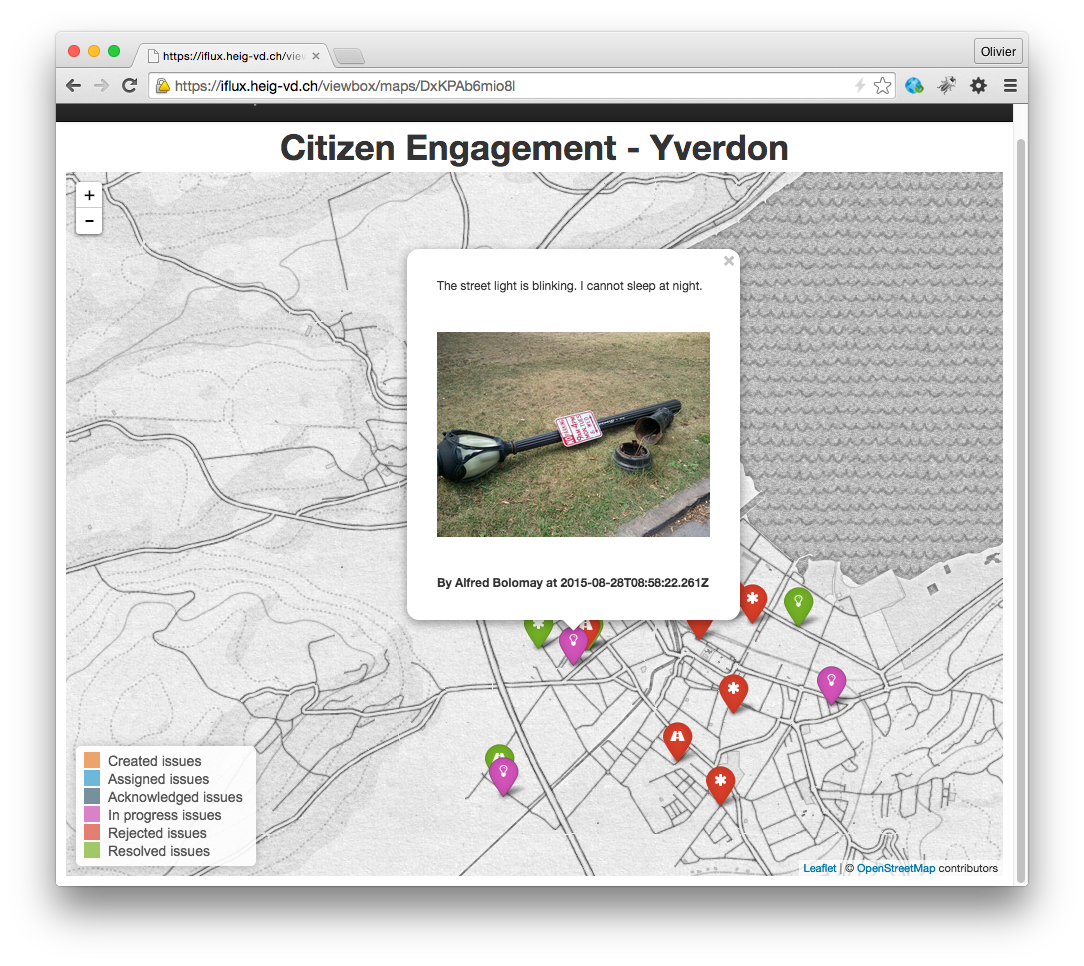
\includegraphics[width=0.9\columnwidth]{figures/citizen-viewbox.png}
\caption{Issues shown by the ViewBox action target}
\label{fig:citizenMap}
\end{figure}

As illustrated in Figure \ref{fig:citizenMap}, we were then able to combine the new \emph{event source} with existing \emph{action targets}. It was really easy to implement a workflow to notify city staff about new issues, either via Slack or via email. It was also very easy to create a map to visualize the issue with the \emph{Viewbox action target} described before. Figure \ref{fig:citizen} shows the end-to-end workflow in iFLUX. Several rules have been added to trigger behavior in the action targets whenever an issue is updated.

We already provided a full list of examples to configure the \emph{event sources} and \emph{action targets} that we will not do it again for this use case. In place, we will focus on the different events that the Citizen backend will send to iFLUX. We defined three different types of events:

\begin{itemize}
\item\textbf{Issue creation} is sent when a new issue is created in the system. The event will contain: \emph{issueId, imageUrl, creator, description, state, issueTypeCode, lat, lng, createdOn, updatedOn};
\item\textbf{Issue status change} is sent when an issue changed from one state to another state. The event will contain the same fields than the \emph{issue creation} type;
\item\textbf{Action done} is sent when an action is taken for an issue. For example, a comment is posted on an issue. The event will contain the fields: \emph{type, reason, user, issueId, issue, state, date}.
\end{itemize}

Then, we have three different rules to match these events. We trigger the actions to update the \emph{Viewbox} visualization. In the context of this project, we have built the demonstration with 4 different maps. We setup one Citizen Backend with a data simulator that creates realistic citizen usage in Baulmes, Payerne and Yverdon. On the \emph{Viewbox}, we created 4 \emph{action targets} which represent these three locations plus a global one to get the big picture of what is happening in the area and not only in these cities.

%\begin{figure}
%\centering
%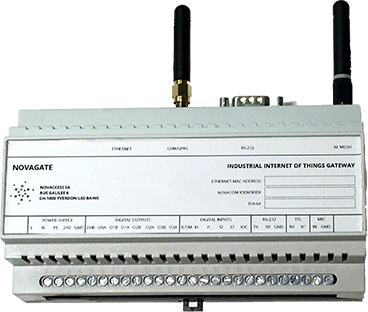
\includegraphics[width=0.8\columnwidth]{figures/novagate.png}
%\caption{The Novaccess IoT gateway is an iFLUX event source}
%\label{fig:novagate}
%\end{figure}


\subsection{Parking @ Paléo}

Paléo Festival is one of the largest music festivals in Switzerland. This year, had the opportunity to evaluate several iNUIT projects in a proof-of-concept deployment. One need expressed by the organizers was to get realtime information about the flow of vehicles and the occupancy of the parkings. To address this question, we created a system composed of one iFLUX \emph{event source} and one iFLUX \emph{action target}. 

The \emph{event source} is a smart object located at the entrance of the parking (see Figure \ref{fig:paleo}), which detects vehicles with ultrasonic sensors. Connected to the Internet via a 802.15.4 mesh network and a WoT gateway, the object emits an event every time a car enters or leaves the parking. The \emph{action target} is responsible for managing application state, which consists of the number of cars currently in the parking, as well as aggregate metrics about the flow of vehicles (number of entries and departures per minute, hour and day). The \emph{action target} publishes this information via a custom REST API, which is used by a web dashboard.

\begin{figure}
\centering
%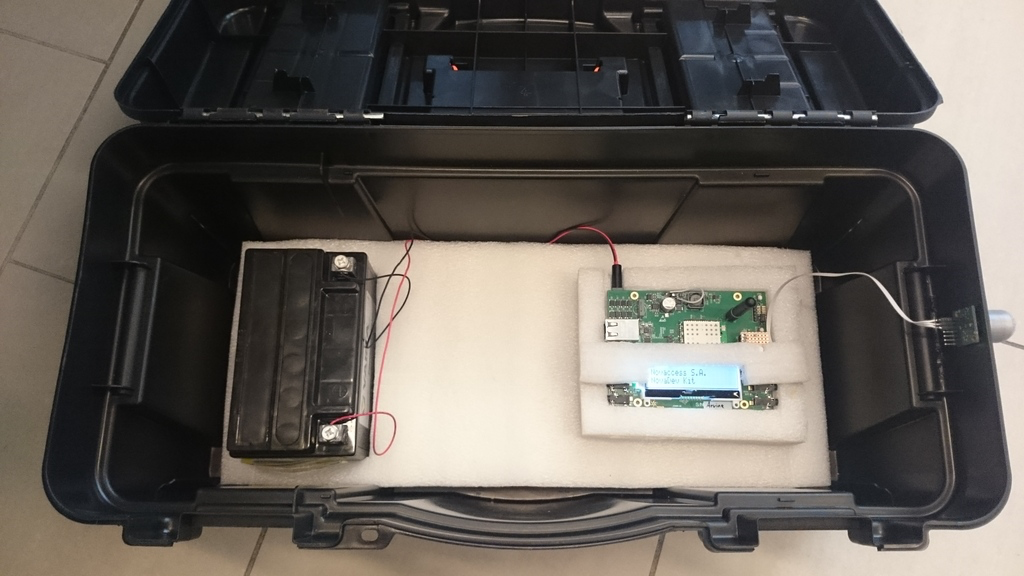
\includegraphics[width=0.9\columnwidth]{figures/paleo-before.png}
%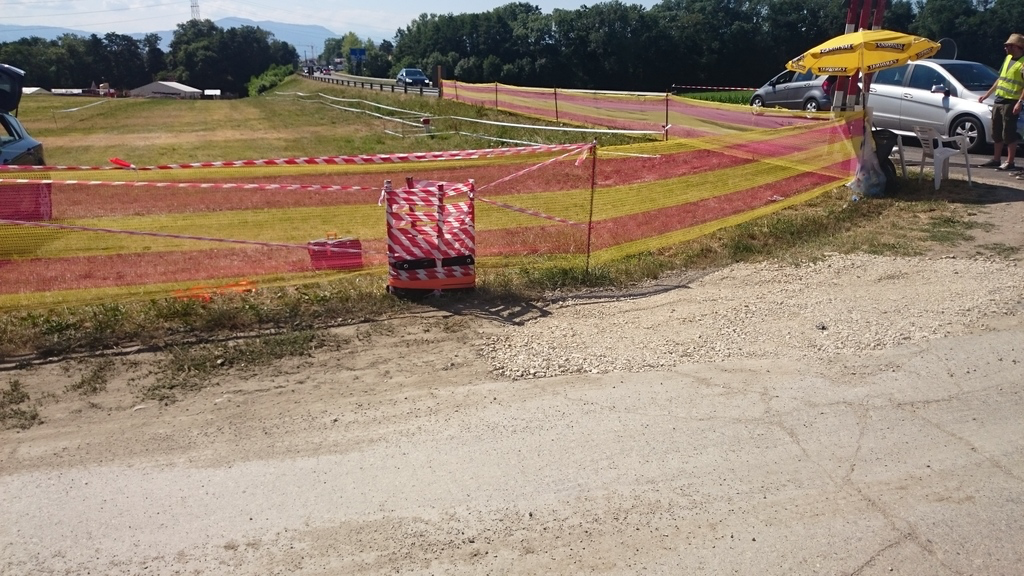
\includegraphics[width=0.9\columnwidth]{figures/paleo-during.png}
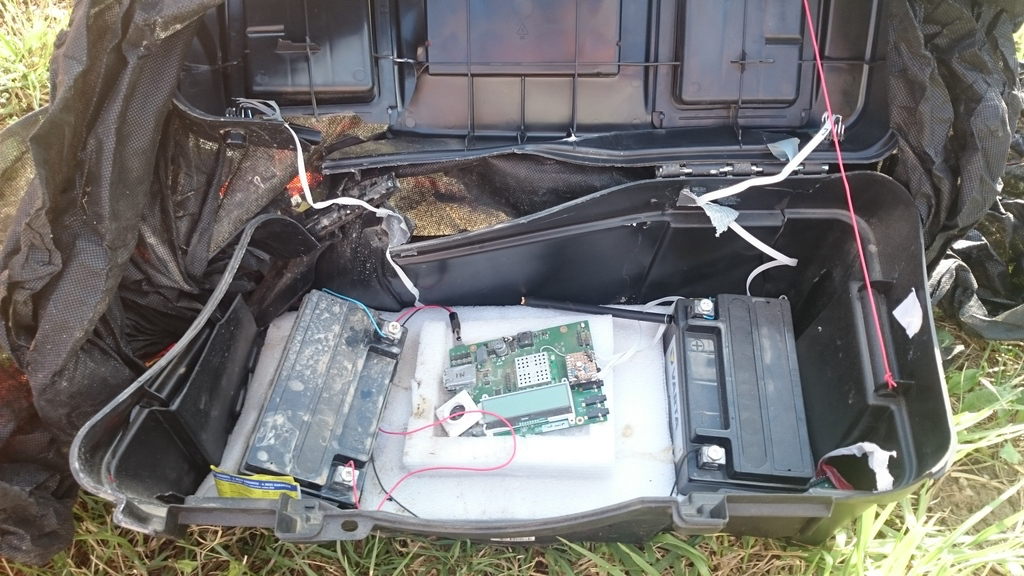
\includegraphics[width=0.85\columnwidth]{figures/paleo-after.png}
\caption{The event source after the festival}
\label{fig:paleo}
\end{figure}

In fact, in this use case, we receive one event every time there is an update. An update means a car which enters the parking or exits the parking. To know if a car comes in or comes out, we have two different sensor which are two different \emph{event sources}. We can build the rules accordingly to that and do the condition from which sensor the event is received. There is an example for the rule for cars in. The rule for exits is very similar to this rule.

\begin{lstlisting}
POST /rules HTTP/1.0
Content-Type: application/json

{
  "name": "Paleo Car In",
  "description": "Detects any cars entering the parking.",
  "active": true,
  "organizationId": 1,
  "conditions": [{
    "description": "Detection done from event source which the sensor dedicated for entrance.",
    "eventSourceId": 3,
  "}],
  "transformations": [{
    "description": "Update the metrics for the Paleo Parking Dashboard",
    "actionTargetId": 3,
    "actionTypeId": 4,
    "fn": {
      "expression": "return { location: event.properties.location, timestamp: event.timestamp };",
      "sample": {
        "event": {
          "location": "westEntry"
        },
        "eventSourceId": 3
      }
    }
  }]
}
\end{lstlisting}

Whit these two rules, we are able to store in a MongoDB some metrics aggregated by minutes, hours, day and months to offer the dashboard presented in Figure \ref{fig:paleoDashboard}. Pay attention that the picture show a simulation of the data. We have developed a data generator for this dashboard to be able to test it.

\begin{figure}
\centering
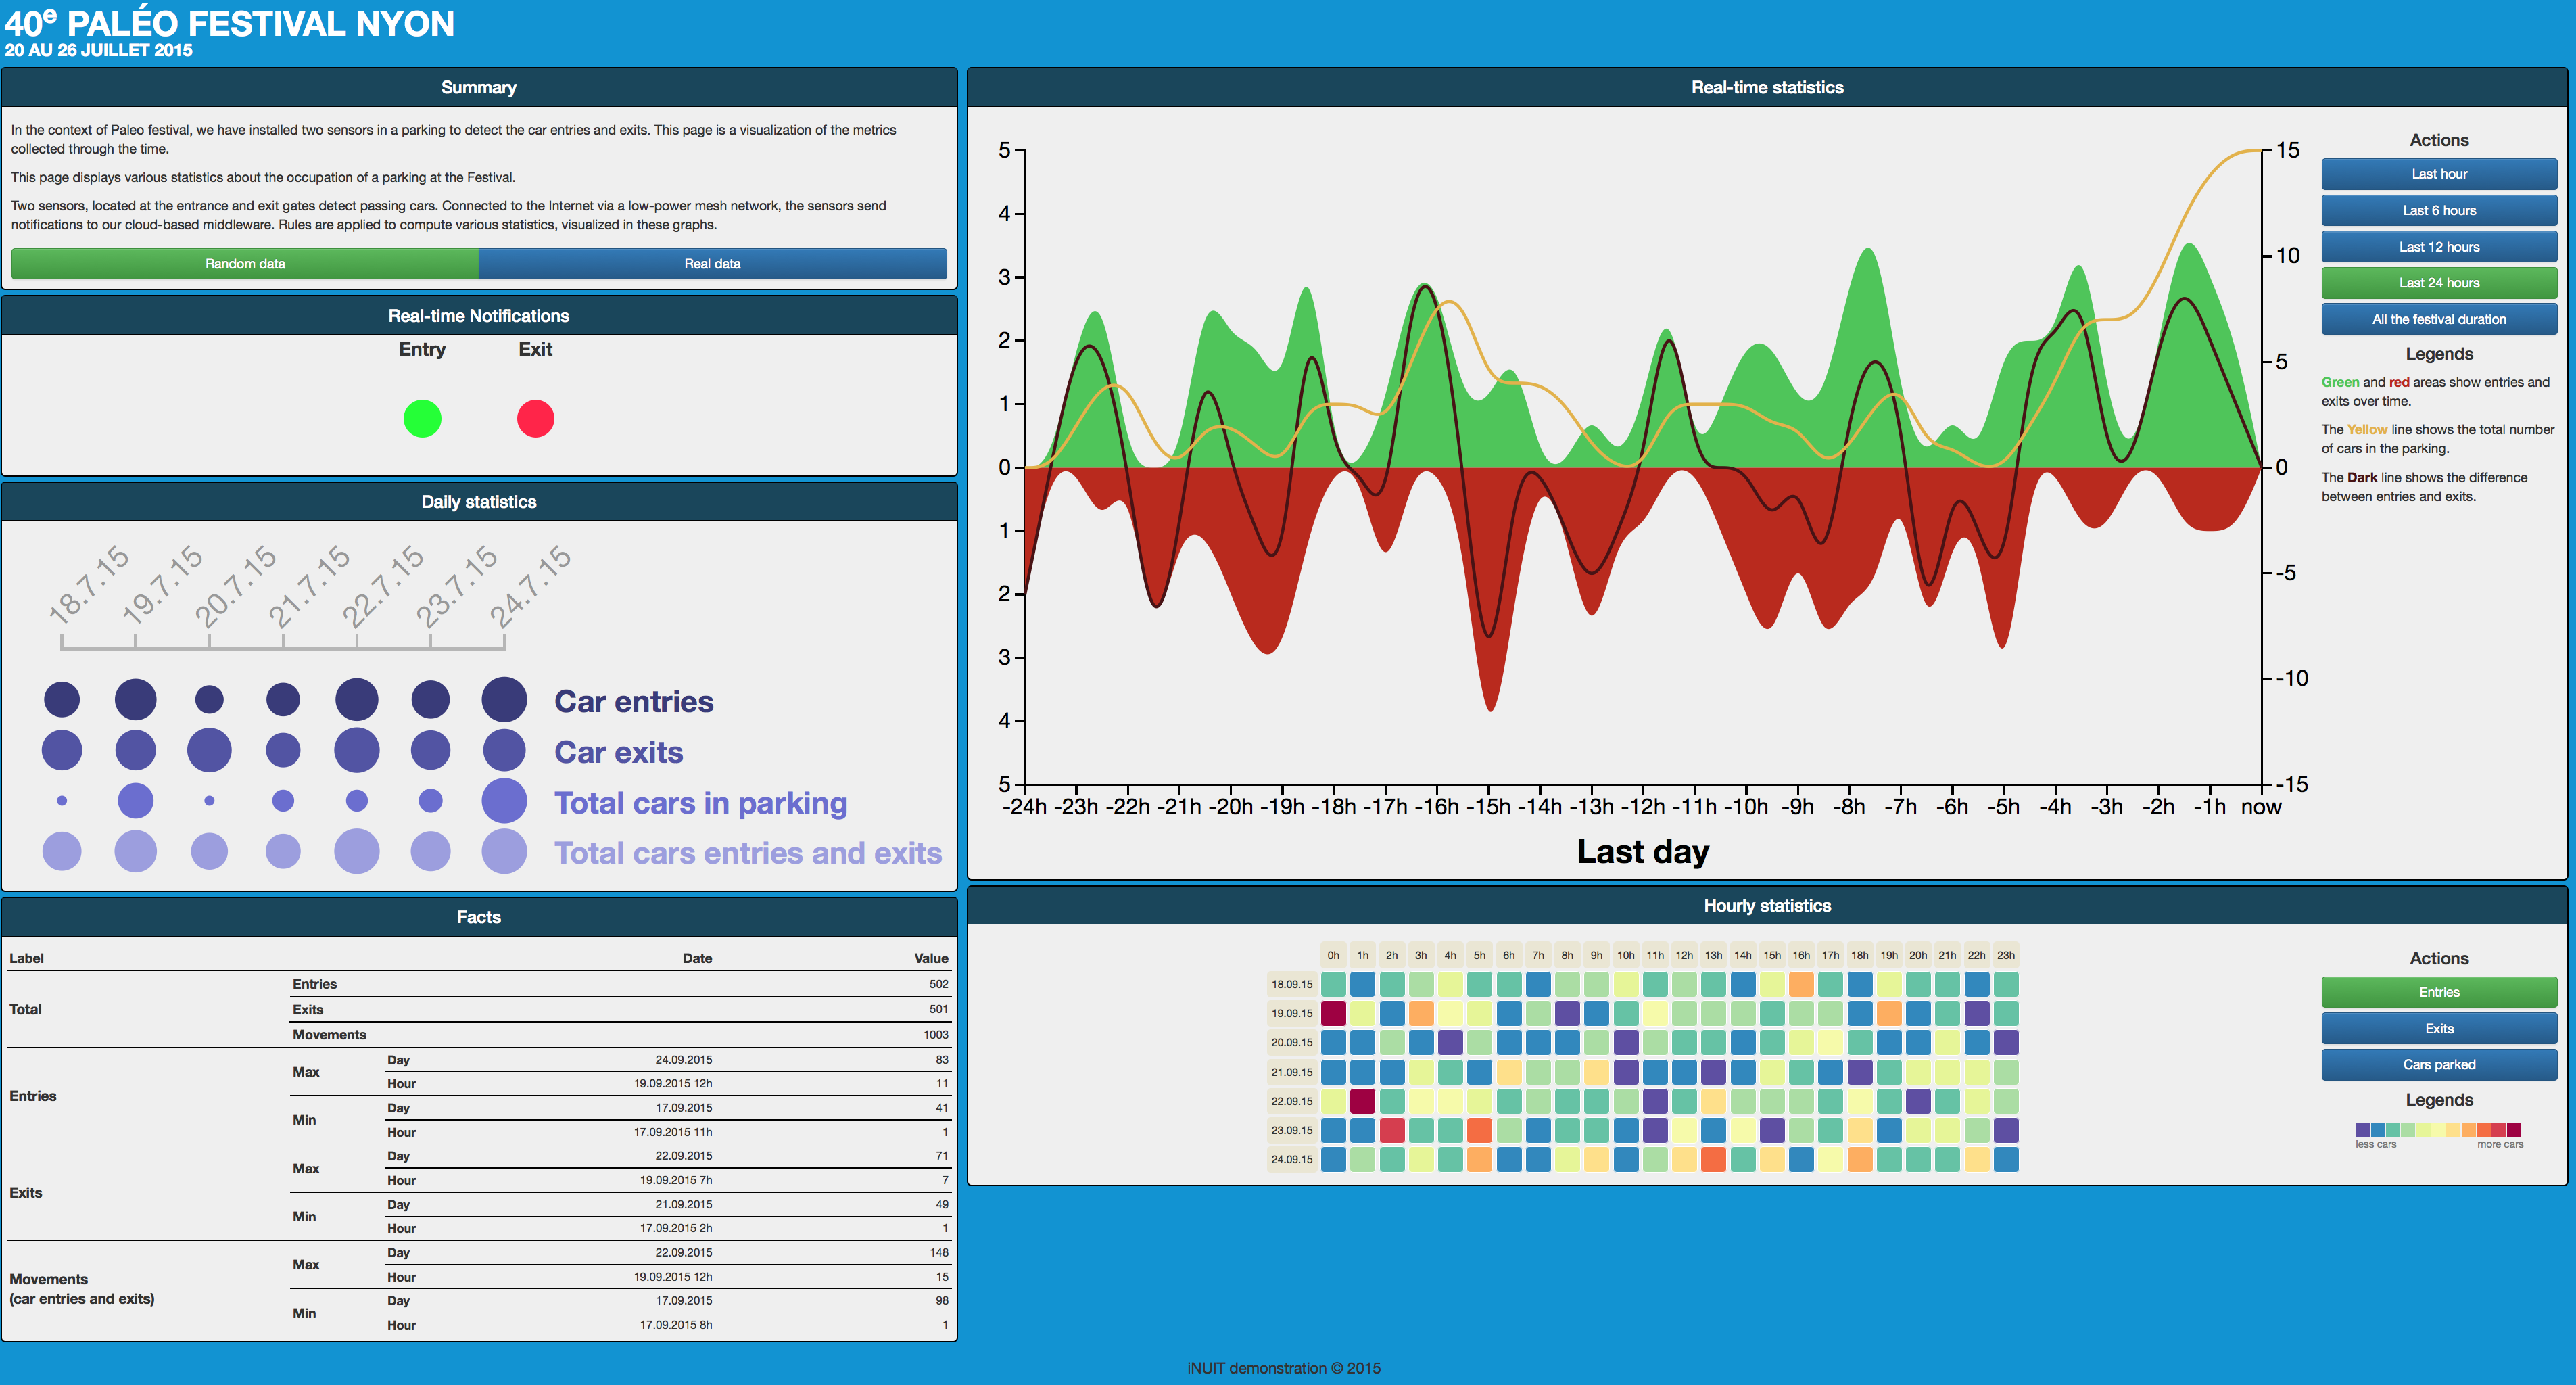
\includegraphics[width=1\columnwidth]{figures/paleoDashboard.png}
\caption{The Paleo Parking Dashboard}
\label{fig:paleoDashboard}
\end{figure}


\subsection{Awareness @ Novaccess}

Novaccess is a startup which develops an integrated stack (hardware, firmware, software) for the industrial Internet of Things. Novaccess has developed NovaLight, a smart lighting solution, which allows municipalities to reduce costs by lowering energy consumption and improving maintenance procedures. Measures are collected from street lights (consumption, faults, etc.) and analyzed. The platform can also dynamically and remotely adjust lighting levels.

%\emph{Awareness} is a concept that has been studied extensively in the Computer Supported Cooperative Work (CSCW) literature. While awareness is a somewhat broad concept, with several definitions, we like to think of it as a general sense of what is happening in a particular environment. In the context of Novalight, \emph{awareness} means that the Novaccess team would like to get a better sense about what is happening, on a continuous basis and without effort. The team would like to be able to detect unusual or interesting patterns. There are actually different dimensions that the team would like to be aware of. For example, Novaccess product owners would like to get a sense of the activity of end-users (are they using the web front-end, are they facing issues, are there features that they use a lot, etc.). Also, Novaccess engineers would like to get a sense of the technical activity (are there communication issues, are there faulty components to replace, what is the amount of transmitted commands, etc.).

We have worked with the Novaccess team to develop an \emph{awareness system} with iFLUX, i.e. a system which collects various types of events and generates notifications for the Novaccess staff. Several \emph{event sources} have been created. The first source, embedded in the NovaLight software, emits events that correspond to user actions (e.g. user has logged in, user has sent a command to a street light, etc.) or to technical issues (e.g. the database size has reached a given threshold). The second source, embedded in the NovaLight IoT gateway, emits events that correspond to measures or technical issues. The \emph{action target} used in the system is the Slack gateway presented before. Rules have been configured on the iFLUX middleware to send the text notifications via Slack, when \emph{interesting} events happen. The flexibility of the setup comes from the fact that it is possible to configure more than a rule. This allows the team to fine tune the amount and destination of the generated awareness messages. This simple setup could easily be extended with other notification devices (lava lamps, color LEDs, etc.).


